\documentclass[12pt]{report}
\usepackage[margin=1in]{geometry}
\usepackage{multicol}
\usepackage{caption}
\usepackage{subcaption}
\usepackage{graphicx}
\usepackage{float}
\usepackage{epstopdf}
\usepackage{setspace}
\usepackage{abstract}
%\usepackage{grffile}
\usepackage{pdfpages}
\usepackage{lscape}
\usepackage{authblk}
\usepackage{hyperref}

\usepackage{fancyhdr}
	\pagestyle{fancy}
	\fancyhead[L]{\today}
	\fancyfoot{}
	\fancyhead[C]{OCE 496 Section 2}
	\fancyhead[R]{\thepage}


\title{\vspace{-5mm}
	\fontsize{20pt}{10pt}\selectfont
	Embedded Wireless Sensor Design for Long Term Structural Health Monitoring
}
		
\author[2]{Christopher Bessin}	
\author[1]{Patrick Blum}
\author[1]{Matthew P. Iannucci}
\author[1]{Jordan T. Kirby}
\author[1]{Zachary McIntosh}
\author[2]{Elizabeth L. Paul}
\author[1]{Michael A. Regan}
\author[2]{Justin W. Skenyon}
\author[1]{Charles J. Wesley}
\author[1]{Samuel D. Wiley}

\affil[1]{Finite Element Modelling}
\affil[2]{Instrumentation Development}
\date{\normalsize\vspace{-3mm}\today}



\begin{document}
\maketitle

%Signature Block

\textit{I have read this paper in its entirety and approve it for submission.}
\vspace{1.5cm}

\noindent\begin{tabular}{ll}
\makebox[2.5in]{\hrulefill} & \makebox[2.5in]{\hrulefill}\\
Christopher Bessin & Date\\[4ex]% adds space between the two sets of signatures
\makebox[2.5in]{\hrulefill} & \makebox[2.5in]{\hrulefill}\\
Patrick Blum & Date\\[4ex]
\makebox[2.5in]{\hrulefill} & \makebox[2.5in]{\hrulefill}\\
Matthew P. Iannucci & Date\\[4ex]
\makebox[2.5in]{\hrulefill} & \makebox[2.5in]{\hrulefill}\\
Jordan T. Kirby & Date\\[4ex]
\makebox[2.5in]{\hrulefill} & \makebox[2.5in]{\hrulefill}\\
Zachary McIntosh & Date\\[4ex]
\makebox[2.5in]{\hrulefill} & \makebox[2.5in]{\hrulefill}\\
Elizabeth L. Paul & Date\\[4ex]
\makebox[2.5in]{\hrulefill} & \makebox[2.5in]{\hrulefill}\\
Michael A. Regan & Date\\[4ex]
\makebox[2.5in]{\hrulefill} & \makebox[2.5in]{\hrulefill}\\
Justin W. Skenyon & Date\\[4ex]
\makebox[2.5in]{\hrulefill} & \makebox[2.5in]{\hrulefill}\\
Charles J. Wesley & Date\\[4ex]
\makebox[2.5in]{\hrulefill} & \makebox[2.5in]{\hrulefill}\\
Samuel D. Wiley & Date\\[4ex]
\end{tabular}

\tableofcontents
\listoffigures
\listoftables

\chapter{Introduction}
	\section{Objectives}
		\subsection{Phase One}
		\subsection{Phase Two}
	\section{Layout}
\chapter{Finite Element Model (FEM)}
	\section{Introduction}
		\subsection{Background of Claiborne Pell Bridge}
		\subsection{Introduction of FEM}
	\section{Abaqus FEM Verification}
		\subsection{L Beam Analysis}
	\section{Claiborne Pell Bridge Model}
		\subsection{Modeling Large Suspension Bridges}
		\subsection{Model Process}
		\subsection{Limitations of Abaqus FEM}

\chapter{Instrumentation Package}
	\section{Introduction}
	\section{Microprocessor}
		\subsection{Necessary Specifications}
		\subsection{Platform Options}
		\subsection{Final Platform}
	\section{Sensors}
		\subsection{Accelerometer}
			\subsubsection{Necessary Specifications}
			\subsubsection{Sensor Options}
			\subsubsection{Sensor Selection}
		\subsection{Strain Gauge}
			\subsubsection{Necessary Specifications}
			\subsubsection{Sensor Options}
			\subsubsection{Sensor Selection}
		\subsection{GPS Receiver}			
			\subsubsection{Necessary Specifications}
			\subsubsection{Sensor Options}
			\subsubsection{Sensor Selection}
		\subsection{CORS}
		\subsection{Analog to Digital Converter}
			\subsubsection{Necessary Specifications}					
			\subsubsection{Platform Options}
	\section{Electronics Design}
			\subsection{Introduction}

\subsection{Circuitry}

\subsection{Printed Circuit Board}
			
	\section{Software Design}
	\section{Package Power}
		\subsection{Power Budget}
		\subsection{Energy Scavenging Potential}
			\subsubsection{Wind Potential}
			\subsubsection{Solar Potential}
		\subsection{Battery Selection}
		
\chapter{Data Collection}
	\section{Phase One Data Collection}
		\subsection{6g Tri-Axial Accelerometer Data}
	\section{Phase Two Data Collection}
		\subsection{6g Tri-Axial Accelerometer Data}
		\subsection{1.5g Tri-Axial Accelerometer Data}
		\subsection{Cell Phone Accelerometer}
		\subsection{Battery Discharge Curve}
		\subsection{Experimental Observed Efficiency}
\chapter{Data Analysis}
	\section{Phase One Data Analysis}
		\subsection{Comparison of Preliminary Abaqus Model and Preliminary Data}
	\section{Phase Two Data Analysis}
		\subsection{Comparison of Developed Abaqus Model with Literature}
		\subsection{Comparison of Developed Abaqus Model with Developed Abaqus Model}	
		
\chapter{Future Development}
	\section{Instrumentation}
		\subsection{Integration of Strain Gauge}
		\subsection{Wireless Transmission}
		\subsection{GPS Time Synchronization}
		\subsection{Package Assembly}
			\subsubsection{Fabrication of Circuit Board}
			\subsubsection{Battery Integration}
			\subsubsection{Package Enclosure}
			\subsubsection{Power Management}
			\subsubsection{Package Location}
	\section{FEM}
		\subsection{Model Improvements}
		\subsection{Dynamic Loading}
\chapter{Conclusion}

\appendix

\chapter{Sensor Package Schematics}
\label{app:Schematic}


\begin{figure}[h]
\centering
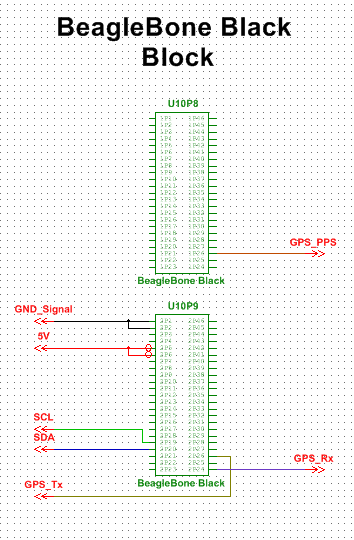
\includegraphics[width=\textwidth,height=\textheight,keepaspectratio]{./KIRBY_Images/Multisim_BBB}
\caption{Schematic of BeagleBone Black}
\label{fig:Schematic_BBB}
\end{figure}

\begin{figure}[h]
\centering
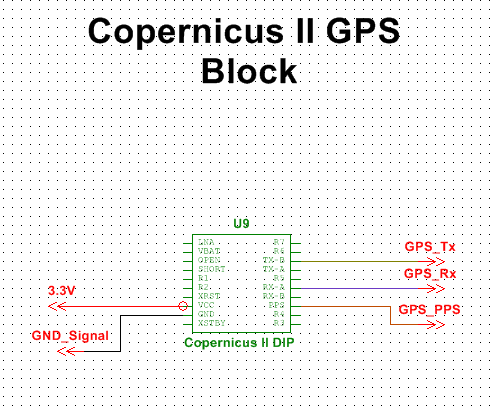
\includegraphics[width=\textwidth,height=\textheight,keepaspectratio]{./KIRBY_Images/Multisim_GPS}
\caption{Schematic of Copernicus II GPS Receiver}
\label{fig:Schematic_Copernicus}
\end{figure}

\begin{figure}[h]
\centering
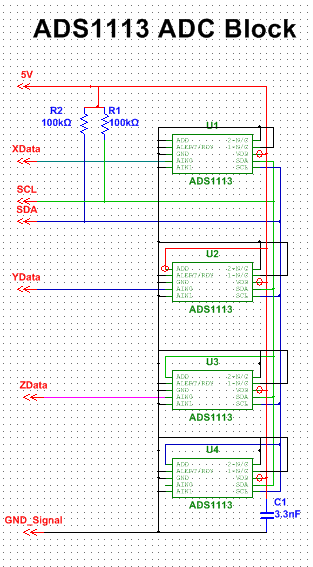
\includegraphics[width=\textwidth,height=\textheight,keepaspectratio]{./KIRBY_Images/Multisim_4ADC}
\caption{Schematic of four ADS1113 ADC units in parallel}
\label{fig:Schematic_ADS1113}
\end{figure}

\begin{figure}[h]
\centering
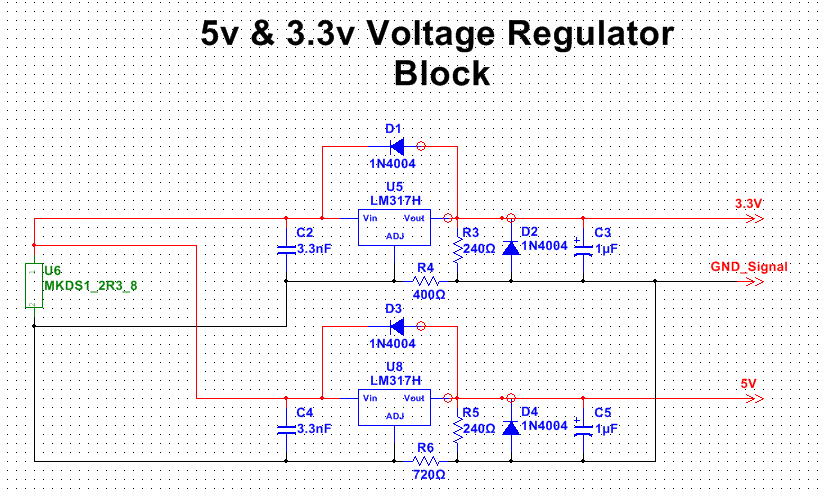
\includegraphics[width=\textwidth,height=\textheight,keepaspectratio]{./KIRBY_Images/Multisim_VoltageRegulation}
\caption{Schematic of 5V and 3.3V voltage regulator circuit}
\label{fig:Schematic_VoltageReg}
\end{figure}

\begin{figure}[h]
\centering
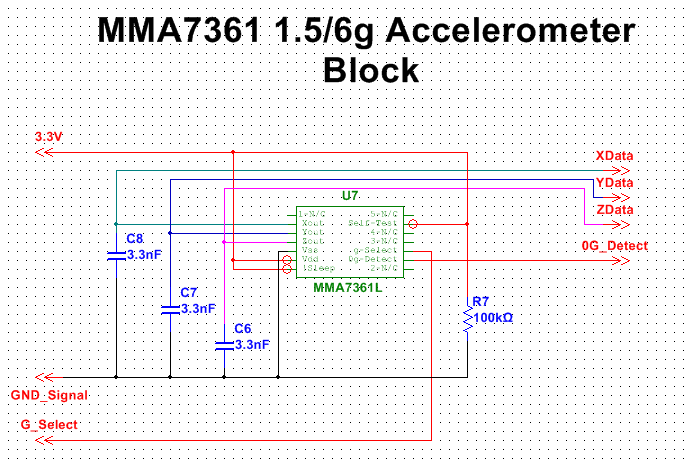
\includegraphics[width=\textwidth,height=\textheight,keepaspectratio]{./KIRBY_Images/Multisim_MMA7361}
\caption{Schematic of MMA7361 $\pm 1.5g/ \pm 6g$ Tri-Axial Accelerometer}
\label{fig:Schematic_MMA7361}
\end{figure}
\end{document}